\chapter
[Bias in estimates of lithosphere viscosity from interseismic deformation]
{Bias in estimates of lithosphere viscosity from interseismic deformation\footnote[1]{
This chapter has been published as: Hines, T. T., and Hetland, E. A.
(2013). Bias in estimates of lithosphere viscosity from interseismic
deformation. Geophysical Research Letters, 40, 4260--4265,
doi:10.1002/grl.50839.}}



\section{Abstract}
The estimation of uniform viscosities representing the lower crust and
uppermost mantle from post- or interseismic deformation (i.e.,
apparent viscosities) is inherently biased with respect to a
depth-dependence of the viscosities within each layer. Estimates are
biased toward a more viscous lower crust or a less viscous
lithospheric mantle, depending on the relative geometric mean
viscosities of the two layers. When there is a low viscosity shear
zone beneath the fault, apparent viscosities are close to that of the
shear zone immediately after the earthquake, although the apparent
viscosities increase significantly during the later interseismic
period.  Inferences made from interseismic deformation that the lower
crust is more viscous than the upper mantle may be entirely consistent
with depth-dependent viscosity profiles that have a significant
increase in viscosity from the lowermost crust to the uppermost
mantle.

\section{Introduction}
Numerous studies in tectonically active regions have sought estimates
of the viscosities of the ductile lithosphere, including the lower
crust and uppermost mantle \citep[e.g.,][]{Hetland2003, Pollitz2003,
Pollitz2005, Johnson2007, Hearn2009}. Here we consider estimates of
the ductile lithosphere made by fitting predictions of surface
deformation from mechanical models to geodetic measurements of
interseismic deformation, including both post- and interseismic
deformation.  Most studies of interseismic deformation concluded that
the lower crust has a higher viscosity than the uppermost mantle
\citep{Burgmann2008, Thatcher2008}. The majority of mechanical models
used in these studies approximated the ductile lithosphere using two
homogeneous viscoelastic layers representing the lower crust and
uppermost mantle \citep[e.g.,][]{Hetland2003,Pollitz2003,Hearn2009}.
These simplistic layered models are commonly used because they are
computationally cheap and because geodetic data are only capable of
resolving a limited number of independent rheologic parameters
\citep[e.g.,][]{Riva2009,Pollitz2010}.  However, the simplifications
made in the layered models may result in inferred viscosities that are
not directly applicable to the real viscosity structure of the ductile
lithosphere \citep{Riva2009}.

Temperature increases with depth and viscosity has a strong
temperature dependence \citep[e.g.,][]{Kohlstedt1995}.  The viscosity
of the ductile lithosphere also has a stress-dependence
\citep[e.g.,][]{Kohlstedt1995}, although the ductile lithosphere is
often approximated as Maxwell viscoelastic in these models
\citep[e.g.,][]{Hetland2003, Johnson2007, Riva2009, Yamasaki2012a}.
This may be a reasonable approximation if stresses resulting from
coseismic deformation are small compared to background stresses.  The
Newtonian viscosity inferred in postseismic deformation studies may
not be constant over time and could be interpretted as an effective
viscosity of a power-law creep \citep[e.g.,][]{Freed2006b}. Indeed, to
describe geodetic observations, models of postseismic deformation in
the months to years following an earthquake often require apparent
viscosities up to several orders of magnitude smaller than those
required in models of deformation later in the interseismic period
\citep[e.g.,][]{Pollitz2005,Johnson2007,Meade2013}. It is important to
note that estimates of viscosities from the first few months following
an earthquake may not be directly applicable to the steady viscosities
of the lithosphere, as the immediate transient postseismic deformation
is often considered to be due to postseismic fault creep, poroelastic
rebound, or a transient rheology \citep[e.g.,][]{Pollitz2003,
Freed2006b, Hearn2009}. We save the investigation of models with
non-linear, power-law creep and/or stress driven fault creep to a
subsequent study, and here we only consider stress-linear
viscoelasticity, allowing for a robust depth-dependence of
viscosities.

We address the question of how inferences of single viscosities
representing the entire lower crust and uppermost mantle are related
to depth-dependent viscosities throughout the ductile lithosphere. We
consider inferred viscosities made from rheologically idealized models
of interseismic deformation to be apparent viscosities, and explore
the biases incurred through using simplified models. For brevity, we
use the term ``strength'' to refer to viscosity, or equivalently
Maxwell relaxation time, $\tau_M$ ($\tau_M = \eta/\mu$, where $\eta$
is viscosity and $\mu$ is shear modulus), and thus we use ``strong''
or ``weak'' to refer to high or low viscosities, respectively. We show
that estimates of the lithosphere's strength, based on simplified
layered models, are almost always biased towards a stronger lower
crust or a weaker upper mantle.

\section{Interseismic models}
We create synthetic surface deformation using 2D earthquake cycle
models composed of an infinite length, vertical strike-slip fault in
an elastic layer of thickness $D$ representing the upper crust,
overlying a Maxwell viscoelastic substrate representing the ductile
lithosphere (Figure \ref{ch1:fig:1}). We impose uniform slip on the
fault with repeat time $T$, until the surface deformation reaches a
cycle invariant state (i.e., the model is spun-up). The lower
viscoelastic substrate is composed of a layer of thickness $D$,
representing the lower crust, and a layer of thickness $8D$,
representing the lithospheric mantle. We choose the thickness of the
latter to be large enough such that the specific thickness does not
affect the surface deformation.  Below $10D$, in the asthenosphere, we
assume a homogeneous viscosity of $10^{19}$ Pa$\cdot$sec to the base
of the model domain.  Models of infinite length, vertical strike-slip
faults are anti-symmetric, and we only model one side of the fault. We
use the finite element program GeoFEST \citep{Lyzenga2000} and take
the model domain to be $120D$ wide by $100D$ deep. We impose an
anti-symmetry boundary condition on the model edge containing the
fault, a far-field velocity, $v_T$, on the opposite boundary, chosen
so that there is no net strain accumulation in each earthquake cycle,
and the top and bottom of the model are stress free (the bottom of the
model domain is sufficiently deep that the bottom stress free boundary
condition does not affect the surface deformation).  We consider only
Maxwell viscoelasticity, but include depth-dependent viscosities
within the lower crust and uppermost mantle. We assume that the shear
modulus is uniform throughout the model and that viscosities vary
smoothly, except possibly at $z = 2D$ (i.e., the Moho) and at $z =
10D$ (i.e., base of the lithosphere).  We non-dimensionalize the
spatial dimensions by the fault locking depth, $D$, and time by $T$,
and thus the non-dimensional Maxwell relaxation time is $\tau =
\tau_M/T$.

\begin{figure}
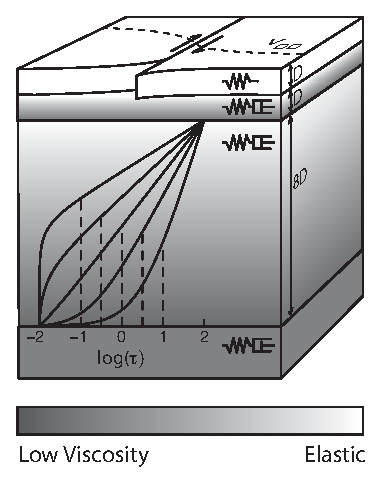
\includegraphics{ch1/figures/Figure1.eps}
\caption
[blerp blerp]
{Schematic of the earthquake cycle model: springs indicate
elasticity and dashpots indicate Newtwonian viscosity. Example
depth-dependent $\tau$ profiles are shown in the upper mantle, for the
case when $\tau^{\min}_{UM} = 10^{-2}$, $\tau^{\max}_{UM} =10^{2}$,
and $\bar{\tau}_{UM}$ indicated by vertical dotted lines.}
\label{ch1:fig:1}
\end{figure}

\subsection{Depth-dependence of $\tau$}
Motivated by the fact that effective viscosity decreases exponentially
with increasing temperature \citep[e.g.,][]{Kohlstedt1995}, we take
$\tau$ to decrease exponentially with depth. For generality, we do not
assume any particular geotherm or composition of the ductile
lithosphere, and instead specify that $\tau$ decreases in each layer
as
\begin{equation}
\tau(z) = \alpha + \beta e^{-\gamma z},
\label{ch1:eq:tau}
\end{equation}
where $z$ is depth within the layer, and $\alpha$, $\beta$, and
$\gamma$ are parameters that vary for each layer.  The parameters in
equation (\ref{ch1:eq:tau}) depend on the maximum, $\tau_j^{\max}$,
minimum, $\tau_j^{\min}$, and geometric mean, $\bar{\tau}_j$,
relaxation times within layer $j$, where $j$ is ``LC'' or ``UM'' for
the lower crust or mantle lithosphere, respectively.  We consider a
wide range of viscosity profiles such that $10^{-1} \leq \tau_j^{\max}
\leq 10^{2}$, $10^{-2} \leq \tau_j^{\min} \leq 10^{1}$, and $10^{-1}
\leq \bar{\tau}_j \leq 10^{1}$, in increments of $10^{0.5}$.  With
these ranges, we consider 5,625 depth-dependent lithosphere viscosity
structures. The relaxation times are non-dimensionalized by $T$, so
for a 100 year recurrence time, the shortest and longest Maxwell
relaxation times we consider are 1 year and $10^{4}$ years,
respectively (corresponding to viscosities of about $10^{18}$
Pa$\cdot$s and $10^{22}$ Pa$\cdot$s for $\mu \approx 30$ GPa).  Note
that we consider profiles both in which the largest decrease of $\tau$
is predominantly in the top or bottom of the layer (Figure
\ref{ch1:fig:1}), and we remark on the impact of this on our results
below.

\section{Determination of apparent strength}
We define the apparent relaxation times (or equivalently the apparent
viscosities) of the lower crust, $\hat{\tau}_{LC}$, and mantle
lithosphere, $\hat{\tau}_{UM}$, as the relaxation times inferred from
surface interseismic deformation using a model composed of constant
viscosities in the two layers (i.e., a layered model). In
general, $\hat{\tau}_{LC}$ and $\hat{\tau}_{UM}$ have a temporal
\citep{Riva2009} and spatial \citep{Yamasaki2012} dependence.  Both of
which can be thought of as variables of interseismic surface
deformation given a particular mechanical representation of the
ductile lithosphere, but here we only consider the time dependence of
inferred viscosities.  We denote the interseismic surface velocities
in the models with depth-dependent $\tau$ as $v_{DD}$, and the
velocities in a layered model as $v_{L}$.  We use a grid search to
determine the $\hat{\tau}_j$ in a layered model that produced surface
velocities that closest match the surface velocities in each of the
depth-dependent models at 100 evenly spaced times throughout the
interseismic period.  In the grid search, we search over $10^{-2} \leq
\hat{\tau}_j \leq 10^2$, minimizing the root mean square error (RMSE)
between $v_{DD}$ and $v_L$ at $0.5D$ increments of distance from the
fault from $0.5D$ to $12D$\@.  We note that the upper limit of
$\hat{\tau}_j$ searched over is a bit excessive because, for practical
purposes, $v_{L}$ is insensitive to changes in relaxation time for
$\tau \gtrsim 10^1$, as the layer is effectively elastic over
interseismic periods \citep{Savage1978} (Figure \ref{ch1:fig:A1}).
Finally, we assume that the fault slip-rate and thickness of the lower
crust and upper mantle are known.

About halfway through the interseismic period, surface deformation for
almost all models we consider, both layered and depth-dependent, is
indistinguishable from the deformation predicted by an elastic model
with slip rate $v_T$ and locking depth $D$ \citep{Savage1973a} (Figure
\ref{ch1:fig:2}A). Because all models simultaneously predict surface
interseismic velocities similar to the elastic model, $\hat{\tau}_j$
cannot be definitively resolved for a period during the middle of the
earthquake cycle (Figure \ref{ch1:fig:3}C). The exact times within the
earthquake cycle in which the elastic model describes $v_{DD}$ as well
as a layered model, depends on the specific $\tau$ profiles, but it is
during the time period about $.4T$--$.5T$ for most of the models.

\begin{figure}
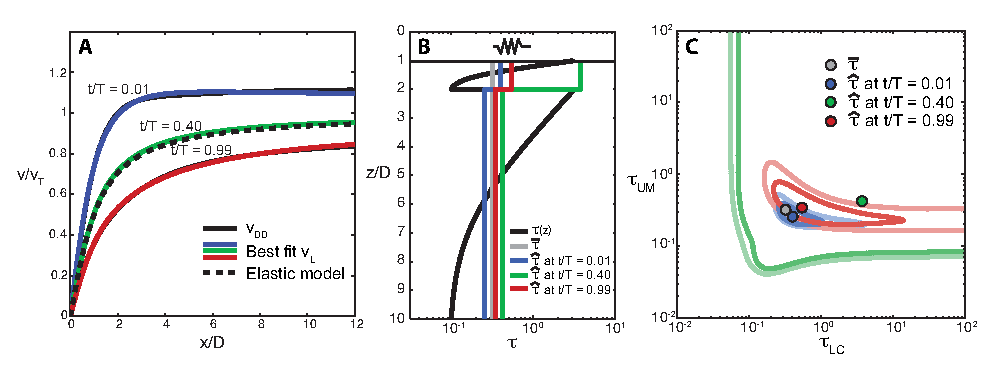
\includegraphics{ch1/figures/Figure2.eps}
\caption{A) Velocities for a depth-dependent model, $v_{DD}$ (black
solid lines) and the best fitting velocities predicted by a layered
model, $v_{L}$ (colored solid lines).  Black dashed line is the
velocities predicted by an elastic earthquake model with the same $D$
and $v_{T}$.  B) $\tau$ profiles corresponding to $v_{DD}$ in (A) and
$\hat{\tau}_j$ associated with the best fitting $v_{L}$ in (A).  C)
$\bar{\tau}_j$ for the $\tau$ profile in (B) with $\hat{\tau}_j$ for
each of the cases in (B). Solid lines indicate misfit contours in the
grid-search estimation of $v_{L}$ in (A); contours shown are RMSE =
0.02 (dark lines) and 0.04 (faded lines), and color indicates the
time.}
\label{ch1:fig:2}
\end{figure}

\begin{figure}
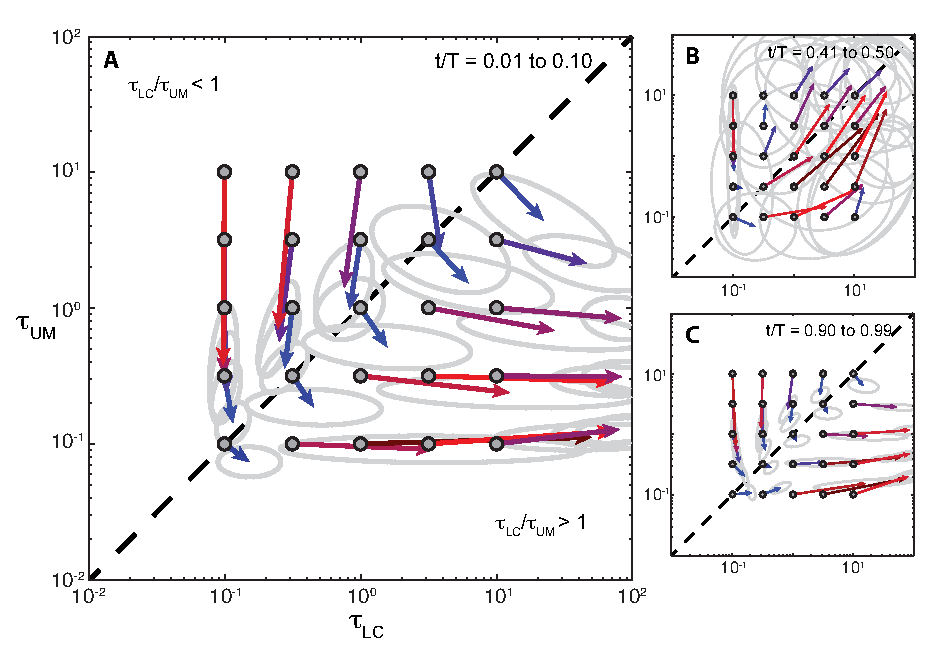
\includegraphics{ch1/figures/Figure3.eps}
\caption{$\bar{\tau}_j$ for all depth-dependent $\tau$ models
considered (gray dots), along with the estimation Bias($\hat{\tau}_j$)
(vectors) early (A), midway (B), and late (C) in the interseismic
period.  Each vector points to the mean $\hat{\tau}_j$ estimated from
depth-dependent models with the same $\bar{\tau}_j$, and the gray
ovals indicate one standard deviation of $\hat{\tau}_j$.  The vector
colors reflect the magnitude of the bias and help to distinguish
overlapping vectors.} 
\label{ch1:fig:3}
\end{figure}

In general, the misfit between $v_{DD}$ and $v_{L}$ is largest early
in the earthquake cycle for models with low $\bar{\tau}_{LC}$ and/or
$\bar{\tau}_{UM}$ (Figure \ref{ch1:fig:A2}). The heightened misfit reflects
the fact that there is more postseismic creep in the mid-crust and/or
beneath the Moho in the layered models, resulting in differences in
the wavelength of surface deformation compared to the depth-dependent
models in which $\tau$ is larger in the mid-crust and/or beneath the
Moho.  Misfit decreases to a minimum halfway into the earthquake cycle
when deformation appears elastic.  The misfit increases again late in
the earthquake cycle, although $v_{L}$ is a significantly better match
to $v_{DD}$ compared to immediately after the earthquake.

We illustrate the determination of $\hat{\tau}_j$ using a model with a
depth-dependent $\tau$ profile such that $\bar{\tau}_{LC} =
\bar{\tau}_{UM} = 10^{-0.5}$, $\tau_{LC}^{\max} = \tau_{UM}^{\max} =
10^{0.5}$, and $\tau_{LC}^{\min} = \tau_{UM}^{\min} = 10^{-1}$ (Figure
\ref{ch1:fig:2}). For this particular case, the misfit surfaces in the
grid search shows clear minima and $\hat{\tau}_j$ is a fair
approximation for $\bar{\tau}_j$ early and late in the interseismic
period, although the lower crust relaxation time is slightly
overestimated (Figure \ref{ch1:fig:2}C). About halfway into the cycle,
the layered model that best fits $v_{DD}$ dramatically overestimates
the lower crust relaxation time (Figure \ref{ch1:fig:2}B); however,
there is a large range of $\hat{\tau}_j$ that would sufficiently match
$v_{DD}$ (Figure \ref{ch1:fig:2}C), since during this period the
surface velocities for all models are very close to the velocities for
the elastic model with identical fault slip rate and locking depth
(Figure \ref{ch1:fig:2}A). In this particular depth-dependent model,
the velocities throughout the interseismic period are quite similar to
those from elastic models, albeit with different slip rates and
locking depths.

\section{Biases in apparent strength}
One might assume that the apparent $\tau$ estimated using a simple
layered model, $\hat{\tau}_j$, reflects the geometric mean $\tau$ in
those layers, $\bar{\tau}_j$. In general, $\hat{\tau}_j$ estimated
from $v_{DD}$ at any time in one of the depth-dependent models may be
significantly different than $\bar{\tau}_j$.  We consider the
difference between the two values to be an error in the estimation of
$\bar{\tau}_j$ and approximate the bias in the estimation throughout
the interseismic period as
\begin{equation}
\mathrm{Bias}(\hat{\tau}_j; \bar{\tau}_j) = E[\hat{\tau}_j] - \bar{\tau}_j,
\label{ch1:eq:bias}
\end{equation}
where $E[\hat{\tau}_j]$ is the geometric mean of $\hat{\tau}_j$
estimated from the collection of the depth-dependent models that all
have the same $\bar{\tau}_j$.

$\mathrm{Bias}(\hat{\tau}_j; \bar{\tau}_j)$ represents the bias in the
estimated relaxation times for the lower crust and uppermost mantle
with respect to the geometric mean relaxation time of the two layers.
In the wide range of models we considered, the bias depends on the
contrast between the geometric mean relaxation times in the lower
crust and upper mantle, $\bar{\tau}_{LC} /\bar{\tau}_{UM}$.  Early and
late in the earthquake cycle there is a distinct bias towards an
apparently weak upper mantle when $\bar{\tau}_{LC} / \bar{\tau}_{UM} <
1$ and a bias exaggerating the strength of the lower crust by up to a
few orders of magnitude when $\bar{\tau}_{LC} / \bar{\tau}_{UM} > 1$
(Figure \ref{ch1:fig:3}A,C).  About halfway through the interseismic
period, the biases we calculate are not well constrained, but are
generally towards a stronger lower crust and uppermost mantle (Figure
\ref{ch1:fig:3}B). These biases hold when we only consider $\tau$
profiles in which $\tau$ decays with depth faster than log-linearly
(Figure \ref{ch1:fig:A4}), which indicates the biases are not sensitive to
the specific decay of viscosity with depth provided that there is
still some depth-dependence within both layers.

When we consider models in which the lower crust is homogeneous, and
include a depth-dependent $\tau$ only in the uppermost mantle, there
is no clear bias when $\bar{\tau}_{LC} / \bar{\tau}_{UM} < 1$.
However, when $\bar{\tau}_{LC} / \bar{\tau}_{UM} > 1$, there is a bias
to a stronger lower crust and only a slight bias in the upper mantle
strength (Figure \ref{ch1:fig:A3}A,C).  Conversely, when the
uppermost mantle has a uniform relaxation time and $\tau$ is
depth-dependent only in the lower crust, there is no bias when
$\bar{\tau}_{LC} / \bar{\tau}_{UM} > 1$, but when $\bar{\tau}_{LC} /
\bar{\tau}_{UM} < 1$ there is a bias towards a weaker upper mantle,
while the lower crust relaxation time is accurately represented
(Figure \ref{ch1:fig:A3}D,F). This may be counterintuitive, as one might
think that if the lower crust or mantle was truly homogenous with
respect to its relaxation time, then a simplified layered model should
accurately capture that uniform relaxation time. In the case of both
the lower crust and uppermost mantle being homogeneous, this would be
true. However, if only one layer has a homogeneous relaxation time
which is longer than the mean relaxation time in the depth-dependent
layer, then strength estimates for that layer are biased.  This leads
us to conclude that the biases are created by the depth-dependence of
$\tau$ in the weaker of the two ductile lithospheric layers.

\section{Lower crustal shear zones}
It is likely that highly sheared rocks directly beneath a fault are
considerably weaker than the surrounding lower crust
\citep[e.g.,][]{Montesi2003}, and lower crustal shear zones are well
documented \citep[e.g.,][]{Vauchez2003}. In all of the models that we
present above, the largest $\tau$ in the lower crust is immediately
beneath the fault.  These long relaxation times may suppress the
relaxation of coseismic stresses in the lowermost crust, where the
relaxation times are shorter, and thus may significantly influence our
above conclusion that estimates of lower crustal strength are biased
to stronger values than its geometric mean strength. To investigate
the potential effect of a lower crustal shear zone on the biases in
$\hat{\tau}_j$, we include a $D$ wide vertical shear zone extending
through the lower crust beneath the fault.  We assume that the shear
zone is Maxwell viscoelastic with a constant relaxation time of
$\tau_{SZ} = 10^{-2}$, which is at least an order of magnitude faster
than the surrounding lower crust.

With a weak shear-zone, immediately following an earthquake the
velocities are quite large, and as a result both the lower crust and
uppermost mantle appear uniformly weaker than their geometric mean
strength, with $\hat{\tau}_{LC}$ close to $\tau_{SZ}$ (Figure
\ref{ch1:fig:4}). These heightened postseismic velocities decay
rapidly, although how $\hat{\tau}_{LC}$ or $\hat{\tau}_{UM}$ increases
over time depends on $\bar{\tau}_{LC}/\bar{\tau}_{UM}$. If
$\bar{\tau}_{LC}/\bar{\tau}_{UM} > 1$ then $\hat{\tau}_{LC}$ increases
by orders of magnitude, exceeding $\bar{\tau}_{LC}$ (Figure
\ref{ch1:fig:4}B). Otherwise, $\hat{\tau}_{UM}$ rapidly increases
early in the cycle. For all models, $\hat{\tau}_j$ evolves towards a
more reasonable approximation of $\bar{\tau}_j$ late in the cycle
(Figure \ref{ch1:fig:4}B). Additionally, the velocities are relatively
steady throughout the later interseismic period compared to a model
without a shear zone but with similar heightened postseismic
velocities (Figure \ref{ch1:fig:4}A).

\begin{figure}
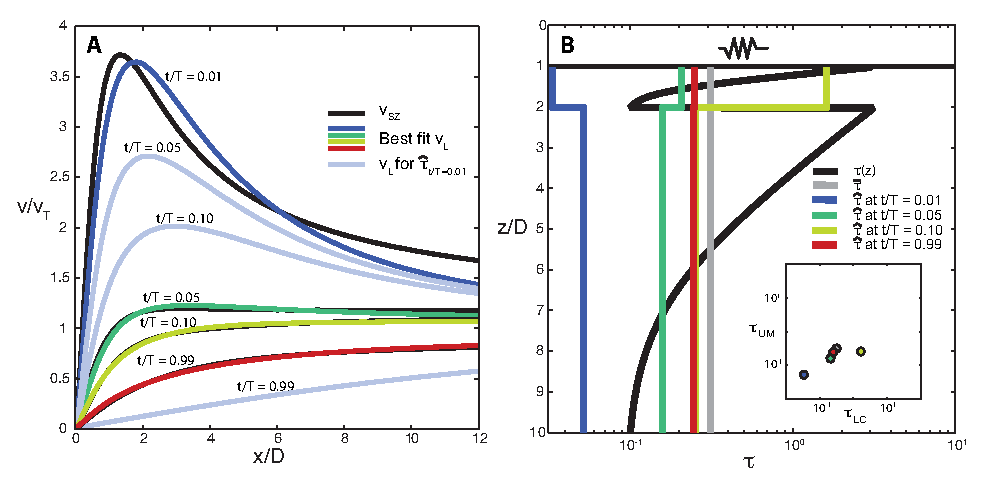
\includegraphics{ch1/figures/Figure4.eps}
\caption{A) Interseismic velocities, $v_{SZ}$, in a model with both a
lower crustal shear zone and depth-dependent $\tau$ in the surrounding
lithosphere (black lines) along with the best fit $v_{L}$ (colored
lines).  Shown as light blue lines are the velocities in a layered
model with the dark blue viscosity profile shown in (b), which are the
apparent viscosities estimated from $v_{SZ}$ at $t/T = 0.01$.  B)
$\tau$ profile outside of the shear zone corresponding to $v_{SZ}$
(black line; $\tau$ = $10^{-2}$ within the shear zone), $\bar{\tau}$
outside the shear zone, and $\hat{\tau}_j$ associated with the best
fitting $v_{L}$ in (A) (colored lines, color corresponds to time in
cycle). Inset in (B) shows $\bar{\tau}_j$ and $\hat{\tau}_j$ (dot
color corresponds to line colors in (A) and (B)).}
\label{ch1:fig:4}
\end{figure}

\section{Discussion}
In the wide range of cases we consider, the biases in $\hat{\tau}_j$
inferred throughout the interseismic period almost always are such
that $\hat{\tau}_{LC}/\hat{\tau}_{UM}$ is larger than
$\bar{\tau}_{LC}/\bar{\tau}_{UM}$, except for midway through the
interseismic period when all velocities are close to the elastic limit
(Figure \ref{ch1:fig:3}B).  Additionally, $\hat{\tau}_{LC}$ is often
larger than $\tau^{\max}_{LC}$ and $\hat{\tau}_{UM}$ is often lower
that $\tau^{\min}_{UM}$.  In models where $\bar{\tau}_{LC} \ne
\bar{\tau}_{UM}$, inferences of $\hat{\tau}_{LC}/\hat{\tau}_{UM}>1$
($<1$) correspond to models in which
$\bar{\tau}_{LC}/\bar{\tau}_{UM}>1$ ($<1$). In other words, a lower
crust that appears stronger than the mantle when approximated by
uniform strength layers corresponds to models in which the geometric
mean strength of the lower crust is also stronger than that in the
mantle, and vice versa.  We note that several of the $\tau$ profiles
with $\bar{\tau}_{LC} > \bar{\tau}_{UM}$ are characterized by
significant portions of the lowermost crust having much lower
viscosities than the uppermost mantle.

The biases we present in this paper can be viewed as relating
$\hat{\tau}_j$ to $\bar{\tau}_j$.  However, the specific relationship
between $\hat{\tau}_j$ and $\bar{\tau}_j$ depends not only on the
details of how $\tau$ varies in the ductile lithosphere, but also on
the time in the interseismic period. In the latter regard, it is also
important to note that we have assumed periodic offsets on an infinite
length fault, whereas real earthquakes are non-periodic and finite. It
is also important to note that we grouped all $\tau$ profiles
according to the $\bar{\tau}_j$ in each layer irrespective of
$\tau^{\max}_j$ and $\tau^{\min}_j$, and only considered how profiles
with the same $\bar{\tau}_j$ relate to $\hat{\tau}_j$.  For these
reasons, these biases cannot be used to back-out specific
depth-dependent $\tau$ profiles, or even unique $\bar{\tau}_j$,
consistent with $\hat{\tau}_j$ estimated from geodetic data using a
simplified model of the lithosphere.  The coherency of the bias
estimates suggest that it may be possible to develop probabilistic
relationships between $\hat{\tau}_j$ and $\bar{\tau}_j$, assuming that
the general time within the earthquake cycle the geodetic data are
sampling is known.  For example, if $\hat{\tau}_{LC} \approx 10^{1}$
and $\hat{\tau}_{UM} \approx 10^{-1}$ were inferred from geodetic data
late in a seismic cycle, then those estimates would be equivalent to
depth-dependent $\tau$ profiles with $\bar{\tau}_{LC}$ around
$10^{-0.5}$ to $10^{1}$ and $\bar{\tau}_{UM}$ on order of $10^{-1}$
(Figure \ref{ch1:fig:3}C). Further exploration of the relationships
between specific $\tau$ profiles and $\hat{\tau}_j$ would be required
in order to establish whether inferences of apparent strength could be
used to constrain the range of permissible $\tau$ profiles that are
consistent with surface deformation at any one time.  It may also be
possible to constrain depth-dependent $\tau$ profiles by considering
how inferred viscosities vary as a function of distance from the fault
\citep{Yamasaki2012}.

In the depth-dependent $\tau$ models we consider, the postseismic
velocities are either only slightly above the elastic velocities or
are large but decay over a relatively long portion of the interseismic
period. Both of these cases are in contrast with many observations of
heightened postseismic velocities decaying over on order of a decade
following earthquakes \citep[e.g.,][]{Ergintav2009}. Models including
transient rheologies or power-law creep have been proposed to explain
transient postseismic velocities \citep[e.g.,][]{Pollitz2003,
Freed2006b, Ryder2007}.  Adding a weak shear zone to a model with
depth-dependent $\tau$ and only Maxwell viscoelasticity can also
result in heightened postseismic velocities that rapidly decay over
the postseismic period, while the surface velocities throughout the
majority of the latter interseismic period are only slightly depressed
compared to those in an elastic model with identical slip-rate and
locking depth (Figure \ref{ch1:fig:4}A).

\section{Conclusions}
Assuming a uniform viscosity for the lower crust and uppermost mantle
results in biased estimates of viscosity for those two layers if the
viscosity is highly depth-dependent.  Estimates of viscosity tend to
be biased either towards a weaker upper mantle or a stronger lower
crust, depending on the relative viscosity of the two layers.  When
there is a low viscosity lower crustal shear zone present, immediately
after the earthquake the lower crust and uppermost mantle both appear
weak, with apparent viscosities close to that of the shear zone, and
then the apparent strength of the lower crust or upper mantle
increases dramatically over the early interseismic period.  Using
simplified models, inferences made from interseismic deformation that
the lower crust is orders of magnitude more viscous than the upper
mantle may be entirely consistent with depth-dependent viscosity
profiles that have smaller contrasts between the geometric mean
viscosities of lower crust and upper mantle and may be associated with
a significant increase in viscosity across the Moho.

\section{Acknowledgments}
This research was funded by NSF grant EAR 1045372. We thank editor E.
Calais, G. Houseman, and an anonymous reviewer.

%\bibliographystyle{agu04}
%\bibliography{refs}

\section{Supporting information}
The following figures provide additional information supporting our
conclusions regarding the biases in apparent viscosities estimated for
the lower crust and upper mantle. The sensitivity of surface
deformation to viscosities in the lower crust or upper mantle is shown
in Figure \ref{ch1:fig:A1}.  Figure \ref{ch1:fig:A2} is the same as
Figure \ref{ch1:fig:3}, except Figure \ref{ch1:fig:A3} also shows all
of the $\hat{\tau}$ for the lower crust and uppermost mantle estimated
from $v_{DD}$ for all models, as well as indicates the misfit of the
associated $v_L$ to $v_{DD}$. Figure \ref{ch1:fig:A3} shows the bias
for end-member scenarios when only the lower crust or upper mantle has
a depth dependent tau. Figure \ref{ch1:fig:A4} shows the bias when tau
in the lower crust and upper mantle has a high decay rate (i.e., a
decay rate larger than a log-linear decrease in $\tau$).

\begin{figure}
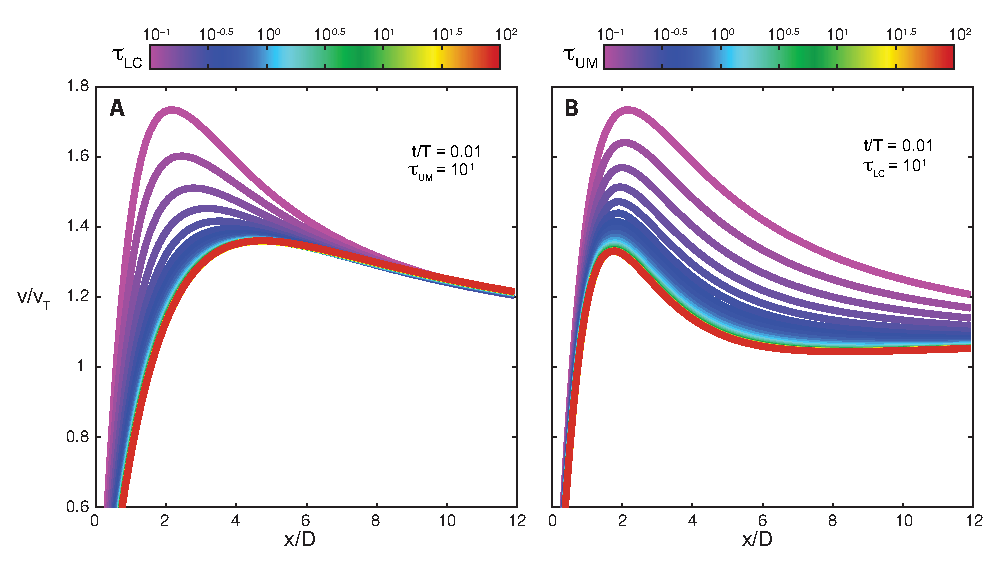
\includegraphics{ch1/figures/AuxFigure1.eps}
\caption{Surface velocities at $t/T = 0.01$ in models with uniform
$\tau$ in the lower crust or uppermost mantle layers ($\tau = \tau_M/T
= (\eta T)/\mu$, where $T$ is the earthquake repeat time, $\tau_M$ is
the Maxwell relaxation time, $\eta$ is the Newtonian viscosity, and
$\mu$ is the elastic shear modulus).  Velocities in models with
constant tau in the upper mantle ($\tau_{UM}$), and variable tau in
the lower crust ($\tau_{LC}$) are shown in (A).  Models with constant
$\tau_{LC}$ and variable $\tau_{UM}$ are shown in (B).  For
sufficiently high $\tau_{UM}$ or $\tau_{LC}$ the surface velocities
converge, indicating that the surface deformation is insensitive to
layer viscosities when $\mathrm{log}_{10}(\tau)$ is above about 1, as
the layer is effectively elastic over earthquake repeat time scales.}
\label{ch1:fig:A1}
\end{figure}

\begin{figure}
\includegraphics{ch1/figures/AuxFigure2.eps}
\caption{$\bar{\tau}_j$ (gray dots) for all depth dependent $\tau$
models considered, along with the estimation of $\mathrm{Bias}(\hat{tau}_j)$,
represented as vectors, early (A), midway (B), and late (C) in the
interseismic period.  Each vector points to the mean value of
$\hat{\tau}_j$ estimated from depth dependent models with the same
$\bar{\tau}_j$.  Colored dots indicate $\hat{\tau}_j$ of each of the best fit
layered models (dot color corresponds to the RMSE of how well $v_L$ fits
$v_{DD}$).}
\label{ch1:fig:A2}
\end{figure}

\begin{figure}
\includegraphics{ch1/figures/AuxFigure3.eps}
\caption{$\bar{\tau}_j$ (gray dots) for all depth dependent $\tau$
models with a homogeneous lower crust (A,B,C) or homogeneous upper
mantle (D,E,F), along with the estimation of $\mathrm{Bias}(\hat{\tau}_j)$,
represented as vectors, early (A), midway (B), and late (C) in the
interseismic period.  Each vector points to the mean value of
$\hat{tau}_j$ estimated from depth dependent models with the same
$\bar{tau}_j$, and the gray ovals indicate one standard deviation of
$\hat{tau}_j$ estimated from models with the same $\bar{tau}_j$.}
\label{ch1:fig:A3}
\end{figure}

\begin{figure}
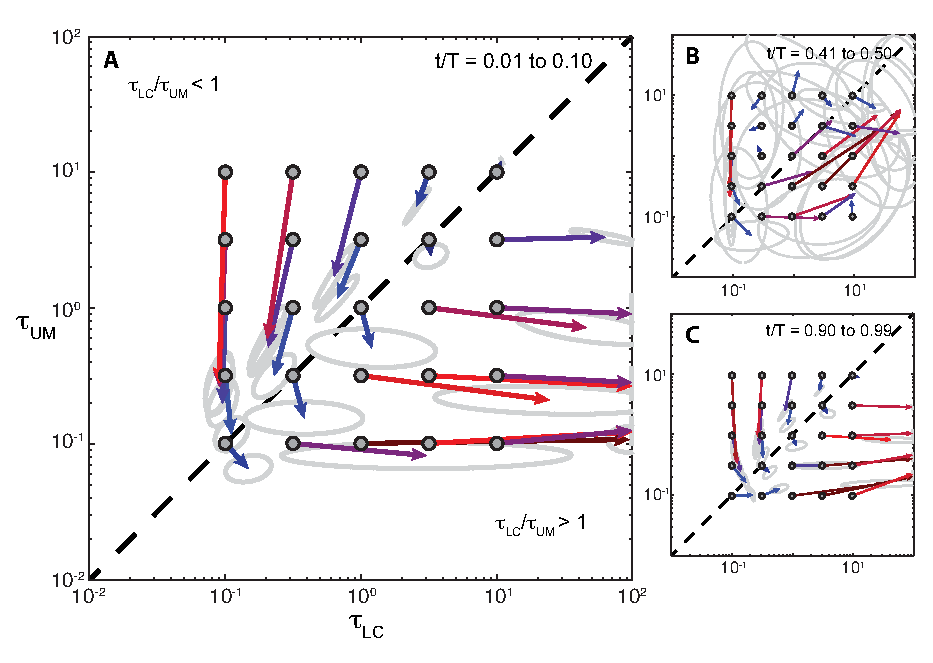
\includegraphics{ch1/figures/AuxFigure4.eps}
\caption{$\bar{\tau}_j$ (gray dots) for all depth dependent $\tau$
models in which $\tau$ in the lower crust and upper mantle decreases
with depth more than log-linearly (i.e., with $\tau$ at any depth
lower than would be predicted by a log-linear decrease, for instance
the left- most $\tau$ profiles shown in Figure \ref{ch1:fig:1}), along
with the estimation of $\mathrm{Bias}(\hat{\tau}_j)$, represented as
vectors, early (A), midway (B), and late (C) in the interseismic
period.  Each vector points to the mean value of $\hat{\tau}_j$
estimated from depth dependent models with the same $\bar{\tau}_j$,
and the gray ovals indicate one standard deviation of $\hat{\tau}_j$
estimated from models with the same $\bar{\tau}_j$.  The estimated
biases in these models are similar to the biases estimated from all
depth-dependent tau models considered in this paper (Figure
\ref{ch1:fig:3}), indicating that consideration of tau profiles that
decay less than log-linearly do not drive our conclusions that the
lower crust (uppermost mantle) appear stronger (weaker) than the
average $\tau$ during much of the interseismic period.}
\label{ch1:fig:A4}
\end{figure}

